\section{Purpose}
\label{sec:numerical-purpose}

Here, we focus entirely on numerical simulations of NLTR as they apply to WPT. Our focus was threefold: (1) to conduct simultaneous NLTR collapses onto two nonlinear objects, (2) to observe the selective collapse of NLTR onto two distinct nonlinear objects, and (3) to characterize the transmission efficiency of the process. From these three focuses, we demonstrated that the NLTR process may be generalized to an arbitrary number of nonlinear objects in an enclosure and that these reconstructions may be selectively rectified at the nonlinear objects. We provide a scheme to characterize the efficiency of our process but were unable to develop a conclusive theory for tuning the efficiency. Our results provide a baseline for developing an experimental algorithm for targeting objects in an enclosure for WPT applications, either selective or non-selectively.  We will first detail the general scheme used for performing NLTR and follow with the setup, experimental results, and discussion for each of our three focus topics.

The process of developing a new technology required benchmarking each step diligently. Any successful WPT technology must have effective transmission efficiency, implying minimal loss in each step of the system. Given the broad frequency signals used in experimentation, a significant drawback to any TR experiment is the inherent wave reflection at interfaces between equipment, various mediums, or circuitry~\cite{smith_waves_2010,griffiths_david_introduction_1999}. While wave reflection losses can be theoretically be measured via S Parameters (explained later) of an experiment, these sources of loss are not practically measurable due to the fact that measuring the losses would create addition interfaces in the system, introducing additional sources of wave reflection~\cite{smith_waves_2010}. To calculate the true ceiling on effective transfer efficiency, it is necessary to numerically simulate the process, as a simulation can calculate the various losses without interfering with the system itself.

In addition to using simulations to study the sources of loss in our system, it also provided us with a simple nonlinear element: a model diode. As explained in previous chapters, the nonlinear response in our \giga experiments was found to be difficult to excite due to power limitations, noise, or equipment sensitivity. The difficulties that we encountered in our physical experimentation were circumvented by numerically simulating the NLTR process. By being able to monitor the voltage and current response of the diode at all times in the simulation, we were able to troubleshoot problems that occurred in the numerical NLTR process that would have otherwise have been impossible to determine in experimentation.

\section{Methodology}
\label{sec:numerical-meth}

\subsection{Equipment}
In order to perform these tests that were not possible in the \giga, we used the program Computer Simulation Technology: Microwave Studio (CST for short) to perform electromagnetic wave simulations. CST is an industry standard modeling program that uses the Finite Integration Technique (FIT) to numerically solve Maxwell's equations~\cite{computersimulationtechnology}. This technique is a generalized version of the well-known Finite Difference Time Domain (FDTD) method but can resolve complex geometries and boundary conditions in a simpler manner. We will not discuss these techniques at length, as they are well-understood in the literature~\cite{schneider2010understanding,weiland2001discrete}.
Our team had two computers with a total of two shared CST licenses to perform simulations. The processing power, RAM, and GPU availability are shown below in Table~\ref{tab:numerical-cpu-specs}. CPU A was used for either single simulations or computationally small simulations. A single simulation refers to a simulation where we did not sweep a parameter.  CPU B was used for large simulations or parameter sweep simulations, requiring either large amounts of memory or large amounts of time, respectively. In general, we used CPU A to perform simultaneous and selective NLTR while we used CPU B to calculate transfer efficiency and characterize nonlinear response characteristics.

\def\arraystretch{2}
\begin{table}[h]
\centering
\begin{tabular}{|l|l|l|}
\hline
 & \textbf{CPU A} & \textbf{CPU B} \\ \hline
Processor & \rule{0pt}{2.5em}\shortstack{Intel Xeon CPU \\ X5670 @ 2.93~GHz} & \rule{0pt}{2.5em}\shortstack{Intel Xeon CPU \\ E5-2680 @ 2.50~GHz} \\ \hline
Number of Processors & 2 & 2 \\ \hline
RAM & 44 GB & 128 GB \\ \hline
GPU Available & No & Yes \\ \hline
\end{tabular}
\caption[Computer specifications]{Technical specifications of the computers used for conducting all simulations and modeling.}
\label{tab:numerical-cpu-specs}
\end{table}

\subsection{Time-Reversal and Nonlinear Sona Extraction}
To start any simulation, we first generated a Gaussian pulse signal in \matlab. For this interrogation signal, we chose the amplitude, center frequency, and bandwidth frequency for our experiment. An example input signal is shown inset in Figure~\ref{fig:numerical-input-wave}. The simulation was run using this pulse signal, noting one of the ports as an injection port (e.g. Port A) and one as the recording port (e.g. Port B).


\begin{figure}[t]
\centering
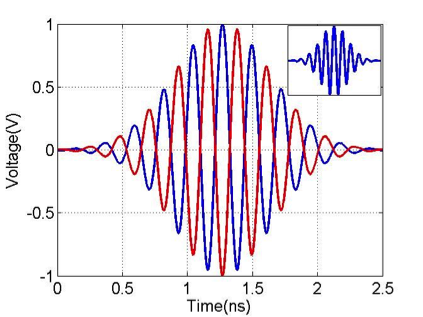
\includegraphics[width=0.85\textwidth]{numerical/input-wave}
\caption[Example of inverted and non-inverted interrogation signals]{This shows our input waveform with a 4.4~GHz center frequency and 1.0~GHz bandwidth. The blue signal is the non-inverted input and the red signal is the inverted input. A singular, non-inverted waveform is shown in the inset.}
\label{fig:numerical-input-wave}
\end{figure}

In general, we had two methods to extract the nonlinear sona from our recorded signal: (1) applying a Fourier transform and band-pass filtering the raw signal and (2) pulse inversion. As previously discussed, many of the \giga experiments were performed by recording a sona, applying a Fast Fourier Transform (FFT), and finally using a band-pass filter on the recorded signals to extract the harmonic signal at the correct frequency. In our numerical simulations; however, the sonas were only recorded for \numrange{30}{35}~ns and the discretized nature of the data on this time scale led to distortion of the sona signals.
The team also explored using pulse inversion, another method of sona extraction that has been well documented in the literature~\cite{simpson_pulse_1999,hong_nonlinear_2014}. Hong et al. have used this method for numerous time-reversal experiments, citing its computational simplicity as a benefit for using it in physical experiments~\cite{hong_nonlinear_2014}. The process involves summing two sonas with inverted inputs.  When the sonas are summed, linear signals are cancelled out, and nonlinear signals remain. Adding the sonas is significantly faster than applying a transformation to an entire sona signal, saving time. While this process proved to be very difficult to implement for our \giga experiments, it was quite efficient at producing the nonlinear sona in CST.
Due to the simplicity of pulse inversion, we used this method for extracting all nonlinear sonas. In this method, we ran the same simulation once with our original input signal and then we ran it a second time with an inverted version of our original signal. Inversion simply means that the entire original signal was multiplied by $-1$. Assuming a linear system, the sum of the original and inverted signals sums to $0$; however, a nonlinear system sum is non-zero. Because the diode is the only nonlinear portion of the system, summing the original and inverted signals yields only the signal from the diode, which is the desired nonlinear sona. Figure~\ref{fig:numerical-sonas}(a) and (b) illustrate two sona signals, where the blue signal is the non-inverted sona and the red signal is the inverted sona. Figure~\ref{fig:numerical-sonas}(b) contains a nonlinear element while~\ref{fig:numerical-sonas}(a) does not. The corresponding (c) and (d) show the result of summing the two signals. It is clear that total annihilation of the sona signal occurs when no nonlinear element is present, as in~\ref{fig:numerical-sonas}(c), while a clear signal is present in~\ref{fig:numerical-sonas}(d).


\begin{figure}[t]
\centering
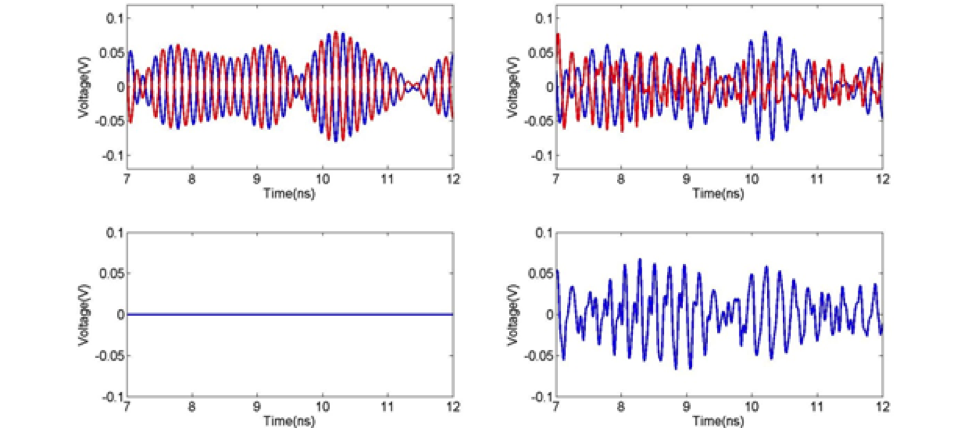
\includegraphics[width=0.85\textwidth]{numerical/sonas}
\caption[Demonstration of pulse inversion]{(a) shows a portion of the non-inverted (blue) and inverted (red) recorded response signal. (b) shows the same two response signals when a diode is present in the simulation. (c) the sum of the two signals in (a), resulting in signal annihilation. (d) the sum of the two signals in (b), which produce a non-zero signal.}
\label{fig:numerical-sonas}
\end{figure}
This method to extract the nonlinear sona was chosen over taking the FFT and filtering the recorded signal as sample rate for the simulation data was not high enough to ensure the results would not be distorted. This discretization of data caused the resulting time-reversed sonas to produce incorrect results using the FFT and filter method, while the time-reversed sonas produced correct results with the pulse inversion method.
\subsection{Defining and Controlling the Nonlinear Element}
In the simulations themselves, we used a model diode as our nonlinear object, as it has a nonlinear I-V curve. The diode location for each simulation was chosen semi-arbitrarily with the only restriction to not be within \numrange{1}{2} wavelengths of either port, as this may have created near-field effects that influenced the results. In CST, the diode component is modeled as the following circuit (Figure~\ref{fig:numerical-cst-diode}) and mathematical relationship (Equation~\ref{eq:numerical-vd-gt-0} and~\ref{eq:numerical-vd-lt-0}). From these, the user may change the parasitic capacitance ($C$), the series resistance ($R$), the reverse conductance ($G_{s}$), and the functional temperature ($T$).

For $V_d > 0$:

\begin{equation}
I_d = I_0\left( e^{\frac{eV_{d}}{kT}-1}\right) = I_0\left( e^{\frac{V_{d}}{V_{k}}a - 1}\right)
\label{eq:numerical-vd-gt-0}
\end{equation}

For $V_d < 0$:

\begin{equation}
I_{d} = G_{s}V_{d}
\label{eq:numerical-vd-lt-0}
\end{equation}


To obtain idealized results, we set $C$ and $G_s$ to $0$, as these values reduced the magnitude of the nonlinear response. We used the default $R = 50 \Omega$, as very large $R$ reduced the overall signal greatly and a very small $R$ did not produce any harmonics. This left only $T$ to tune the I-V curve of the diode. In real life, different diodes have different I-V curves based on material. In order to simulate these differences mathematically, we changed the temperature of the diode in the simulation, as shown in Figure~\ref{fig:numerical-iv-curves}.

In reality, this changed the knee voltage ($V_{k}$) for the diode. We chose $V_{k}$ to be the applied voltage needed to achieve a current of $0.2 I_{0}$. The parameter $a$ is used to define this $0.2 I_{0}$ cutoff. As discussed later in this chapter, we will show how the nonlinear response of a diode is dependent on both the input pulse amplitude and the knee voltage. This nonlinear response was maximized to allow for selective targeting between two diodes simultaneously.
\section{Results}
\label{sec:numerical-results}

\begin{figure}[]
\centering
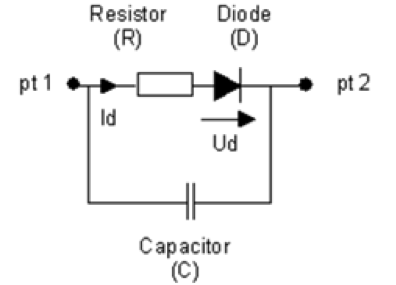
\includegraphics[width=0.7\textwidth]{numerical/cst-diode}
\caption[CST diode circuit model]{CST diode circuit model}
\label{fig:numerical-cst-diode}

\vspace*{\floatsep}% http://tex.stackexchange.com/q/26521/5764

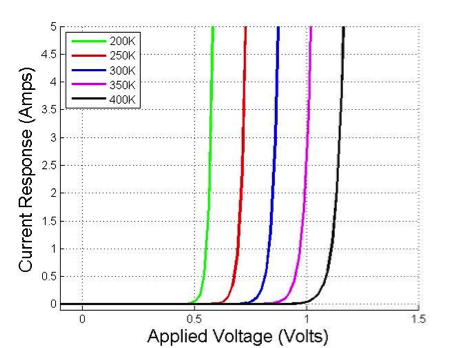
\includegraphics[width=0.7\textwidth]{numerical/iv-curves}
\caption[I-V curves of diodes with different voltage knees]{Different I-V curves that can be modeled in CST. It should be noted that the ``Temperature'' of the diode only changes its mathematical definition of the I-V curve}
\label{fig:numerical-iv-curves}
\end{figure}

\subsection{Simultaneous Nonlinear Time Reversal}

The first focus of our numerical simulations was to illustrate the collapse of a nonlinear time-reversed sona on multiple targets simultaneously. To be an effective WPT system, our technology would need to be able to charge more than one device at a time. Based on literature illustrating NLTR collapsing on a single nonlinear object, we hypothesized that a nonlinear sona would collapse on an arbitrary number of nonlinear objects if the nonlinear objects were present in the time-forward step of NLTR~\cite{nltr-classical-waves,nltr-wave-chaotic}. We assumed that the reconstruction on each nonlinear object would sum linearly and independently such that no reconstruction would interfere with another, as shown in Equation~\ref{eq:numerical-r-tot}, where $R_{i}$ is the reconstruction on a single nonlinear object and $x_{i}$ is a weighting of the amount of power that the single nonlinear object contributes to the overall power of all reconstructions. Based on this, we expected the reconstruction waveforms of the independent single-diode simulations to match a single, multi-diode simulation.

\begin{equation}
R_{tot} = \sum_{i} R_{i}x_{i}
\label{eq:numerical-r-tot}
\end{equation}

This feature was realized by creating a geometry with two diodes present along with two ports to record and emit signals, shown below. We created a quasi-two-dimensional (2D) irregular cavity in CST. This cavity was a 15cm x 15cm x 0.76cm square box modified with various circular and elliptical segments removed from the walls as shown in Figure~\ref{fig:numerical-cst-box}.  The 0.76cm height was chosen to maintain a 2D simulation. Equation~ref{eq:numerical-cutoff-freq} was used to calculate the cutoff frequency for the fundamental mode of a parallel plate cavity, below which only 1 frequency will propagate, reducing the time needed to simulate~\cite{griffiths_david_introduction_1999}.

\begin{equation}
f_c = \frac{c}{2h}
\label{eq:numerical-cutoff-freq}
\end{equation}

Using a cavity of height 0.76 cm resulted in a cutoff frequency of 20~GHz, well above our typical test frequencies of \numrange{4}{5}~GHz fundamental and \numrange{8}{10}~GHz harmonic. We chose this cutoff frequency in the event we needed to use a higher fundamental frequency to create better spatial resolution of our reconstruction. The area dimensions for the Cut Box Model were chosen to minimize computational time while still maintaining a reasonable mode density, as shown in Figure~\ref{fig:numerical-cst-box}(a). This mode density is required to allow the ray chaotic environment to have high sensitivity to initial and boundary conditions; a low mode density will prevent NLTR from having high spatial resolution.

\begin{figure}[t]
\centering
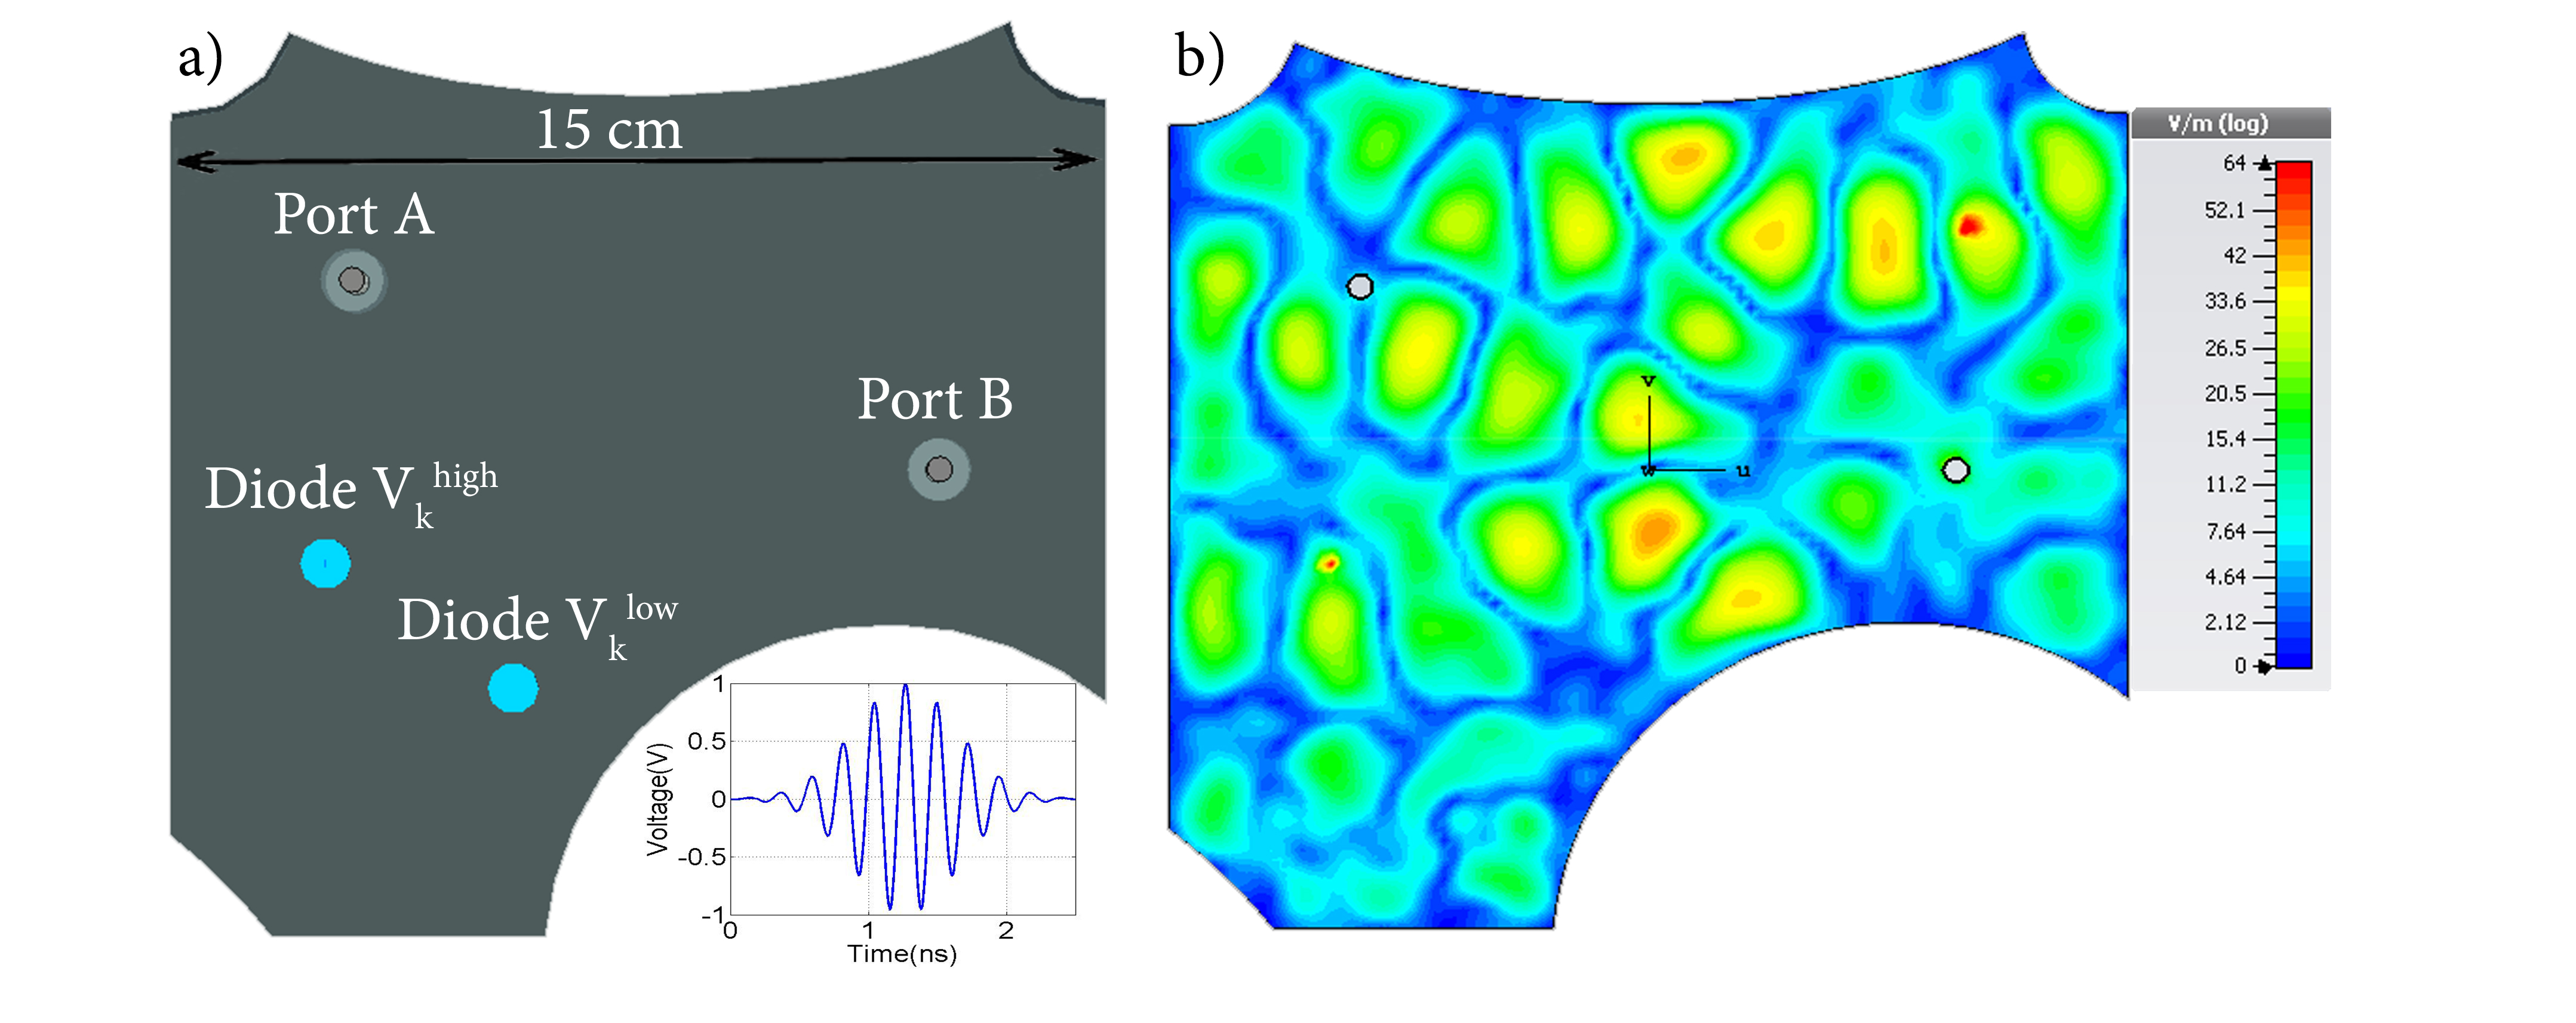
\includegraphics[width=\textwidth]{numerical/cst-box}
\caption[The Cut Box Model]{The Cut Box simulation geometry used in CST. (a) shows the location of the 2 ports (A and B), 2 diodes ($V_k^{high}, V_k^{low}$), length scale, and the lower inset shows the initial interrogation pulse. (b) shows the electric field at a point in the simulation, illustrating the limited excited mode density.}
\label{fig:numerical-cst-box}
\end{figure}

We used two Teflon-coated dipole antennas to emit and record signals~\cite{hemmady2006universal}. Two diodes are placed inside the cavity, shown by the blue circles in Figure~\ref{fig:numerical-cst-box}. A 4.4~GHz center frequency pulse with a 1.0~GHz bandwidth was chosen to minimize the reflected power and applied to antenna A. The interrogating pulse is shown as an inset in Figure~\ref{fig:numerical-cst-box}(a).

The specific frequency and bandwidth was chosen for this geometry to minimize initial wave reflection ($S_{11}$) into the enclosure. Figure~\ref{fig:numerical-s11-spectrum} shows that using a 1.0~GHz bandwidth, an optimal center frequency is 4.4~GHz. The dips in the $S_{11}$ value represent optimal frequencies to use, as a low $S_{11}$ indicates a large portion of the signal entered the cavity. The large number of peaks is indicative of the mode density of the geometry, where low frequencies are sparse given the relatively small scale of the cavity.

\begin{figure}[t]
\centering
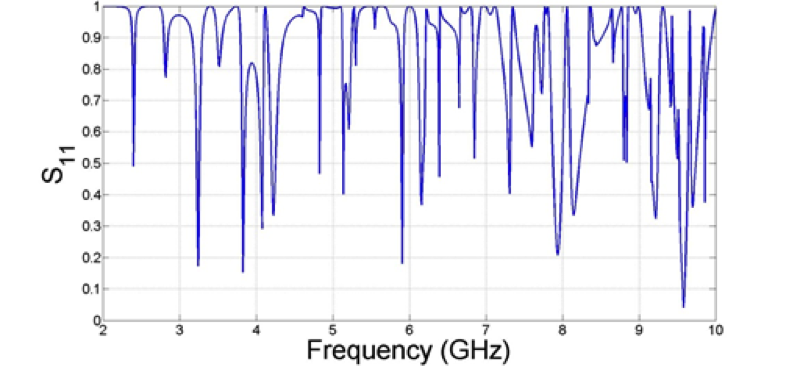
\includegraphics[width=\textwidth]{numerical/s11-spectrum}
\caption[$S_{11}$ spectrum of the Cut Box Model]{The $S_{11}$ spectrum for the Cut Box Model. We wanted to minimize $S_{11}$ for our simulation while maintaining a large bandwidth. This led to choosing a 4~GHz center frequency with a 1.0~GHz bandwidth.}
\label{fig:numerical-s11-spectrum}
\end{figure}

Using this input pulse and the pulse inversion method of sona extraction, we were able to perform NLTR in the Cut Box Model. By measuring the observed voltage and corresponding current during the time-reversed step, we measured the quasi-power over time in each diode. As shown in Figure~\ref{fig:numerical-sim-recon}, the reconstruction waveform on each diode matches the expected results for a 1-diode experiment~\cite{taddese_sensing_2010,barbieri_time_2010}.
\begin{figure}[t]
\centering
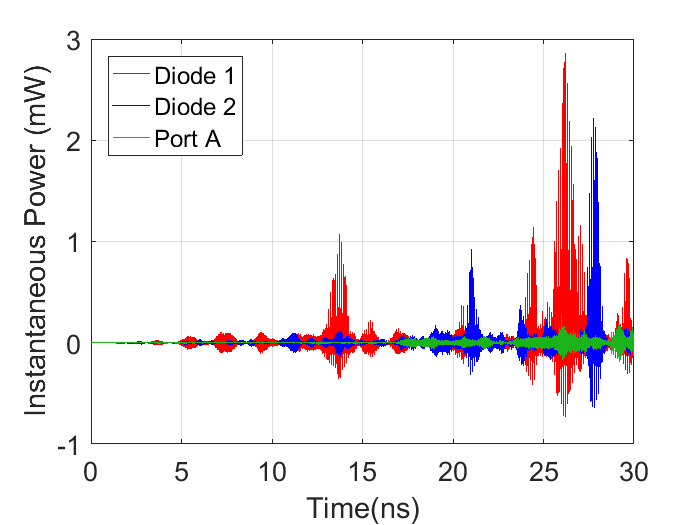
\includegraphics[width=0.75\textwidth]{numerical/sim-recon}
\caption[Simultaneous reconstructions on two diodes]{The time-reversed reconstruction on two diodes simultaneously performed inside the Cut Box geometry.}
\label{fig:numerical-sim-recon}
\end{figure}

\subsection{Discussion of Simultaneous Nonlinear Reconstructions}

This result alone signifies the generality of NLTR whereby any nonlinear object in the cavity will observe a reconstruction in the time-reversed step. In regards to a larger WPT system, one can imagine that this is particularly useful inside of a home or public area, where any device may be powered as long as it is within range of the transmitter/receiver base station. Because the process used only creates a reconstruction at the nonlinear element, it is as simple as repeating the NLTR process rapidly, creating a quasi-pulse width modulation (PWM) signal that can charge a battery. PWM is a method for controlling how active a device is by rapidly switching the device on and off. For example, a fan has different speeds because it operates 25\%, 50\%, 75\%, or 100\% of the time. Similarly, if we can reconstruct on a battery circuit every 10\% or 20\% of the time, we can effectively charge the battery. As soon as the nonlinear object leaves the enclosure, it will no longer receive power. By having a base station that can actively modulate output sona power, it would be very simple to change the amount of power transferred to each device. This dynamic power control is outside the scope of our project but represents a much later extension to this WPT system.

\subsection{Simulation of Selective Collapse of NLTR}
The logical next step is to determine how such a system would be able to determine which device should be powered. As previously shown, if nothing is done to alter the sona signals, then the sona from each nonlinear object will sum linearly and produce a reconstruction at all nonlinear objects in the time-reversed step. Given that each reconstruction sums independent of one another, we hypothesize that we should be able to eliminate the contribution of one nonlinear reconstruction to the overall set of reconstructions without altering the fidelity of any other individual reconstruction on other nonlinear elements. For example, in an enclosure with 3 diodes, if we could suppress the response of diode 2 in the time-forward step, then we would expect to only observe a reconstruction on diodes 1 and 3, creating a selective targeting method. Using Eq. 3, this would imply a weight of $x_{2} = 0$, as shown in Equation~\ref{eq:numerical-r-tot-2}.

\begin{equation}
R_{tot} = \sum_{i}R_{i}x_{i} = R_{1}x_{1} + R_{2}*0 + R_{3}x_{3} = R_{1}x_{1} + R_{3}x_{3}
\label{eq:numerical-r-tot-2}
\end{equation}

In a commercial setting, this would be an extremely useful aspect to our WPT system, as companies could require payment to use the system and would otherwise suppress the reconstruction on the user's device. The fact that the nonlinear object is passive in the environment implies that this selective targeting could even be used to ``resurrect'' a dead phone, a feature not seen on any current WPT technology on the market.

We have developed a method of performing such a targeting scheme based on the previously mentioned diode model. In the simplest case, we show that selective targeting for 2 diodes with two separate voltage knees was obtained (noted $V_k^{high}$ and $V_k^{low}$).

Recall the current response in the diode from Equation~\ref{eq:numerical-vd-gt-0}. One useful aspect to the diode definition function is that if $V < V_{k}$, then the diode has very little current response, which in turn implies a low nonlinear response. We utilize this characteristic while performing selective targeting on a low $V_{k}$ diode. Similarly, we observe that at small $V_{k}$ values, the nonlinear response is small. These two observations led to the hypothesis that nonlinear response may be maximized given an initial pulse by selecting a proper $V_{k}$ value. As shown below, Figure~\ref{fig:numerical-knee-voltages} was obtained by sweeping over many $V_{k}$ values for different initial pulse amplitudes given the same geometry and process conditions as previously stated. Given this distribution, we may target a high $V_{k}$ diode, as the nonlinear response will be stronger in the high $V_{k}$ diode than the low $V_{k}$ diode.

\begin{figure}[t]
\centering
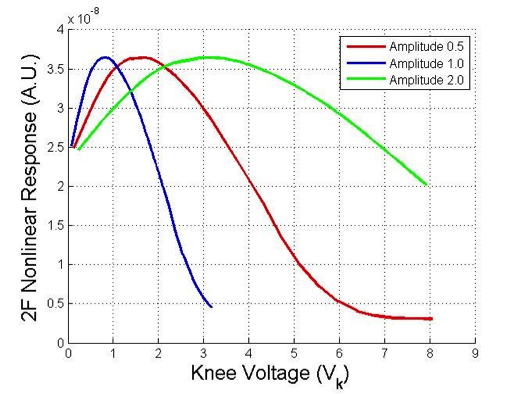
\includegraphics[width=\textwidth]{numerical/knee-voltages}
\caption[Nonlinear response due to different diode characteristics]{The nonlinear response of the diode had a clear maximum at a specific knee voltage. By using a pulse amplitude that corresponded with the specific diode knee voltage, we could selectively target diodes in CST.}
\label{fig:numerical-knee-voltages}
\end{figure}


To perform this selective targeting, we once again used the Cut Box Model. In the simplest case, we consider selective targeting of a low $V_{k} = 0.79V$ ($V_K^{low}$) diode at the exclusion of a high $V_{k} = 6.60V$ ($V_k^{high}$) diode. Given the large value of $V_k^{high}$, we expect to see no response in that diode while maintaining a reasonable nonlinear response in the $V_k^{low}$ diode. We used a pulse with amplitude $V = 1.0 V$ during the time forward step, emitted at Port A in Figure~\ref{fig:numerical-cst-box}(a). Using pulse-inversion, we extracted the nonlinear sona from the recorded signal at Port B, time-reversed the signal, and re-emitted it from Port B. Figure~\ref{fig:numerical-selective-recon-low} shows the time-reversed reconstructions on both diodes. This results in a reconstruction almost exclusively on the $V_k^{low}$ diode during the time-reversed step. The presence of three reconstructions when only one initial pulse was not alarming, as short-orbit paths between Port A, the diodes, and Port B that carry enough power to excite the diode harmonics are known to exist~\cite{hansjurgenstockmann2006}. To calculate the quality of the selective reconstruction, we determined the aspect ratio by comparing the max of $IV$ on both diodes. For this scenario, we calculate a power delivery aspect ratio of 6.35:1 for the $V_k^{low}$ diode relative to the diode with $V_k^{high}$.

\begin{figure}[t]
\centering
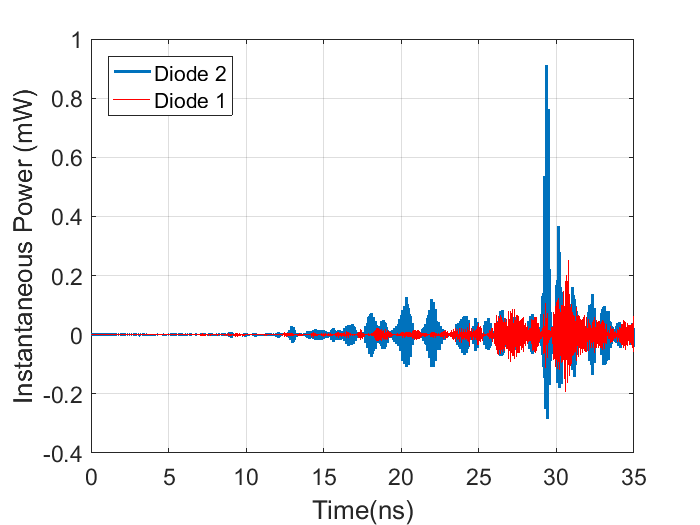
\includegraphics[width=\textwidth]{numerical/selective-recon-low}
\caption[Selective reconstruction on a $V_{k}^{low}$ diode]{Time-reversed reconstructions on the two diodes while targeting $V_{k}^{low}$. Very little signal is seen on the $V_{k}^{high}$ diode. The insert shows the details of the reconstructions between 22 and 30 ns.}
\label{fig:numerical-selective-recon-low}
\end{figure}

 The more difficult scenario was to selectively target a high $V_k$ diode at the exclusion of a low $V_k$ diode. We utilized the peak in nonlinear response as a function of knee voltage from Figure~\ref{fig:numerical-knee-voltages}. By choosing the correct pulse amplitude corresponding to a peak value that was matched to the high $V_k$ value, we expected to see the strongest nonlinear response, resulting in the largest magnitude reconstruction. In this scenario, the low $V_k$ diode still observed a reconstruction; however, it was smaller in amplitude than the high $V_k$ diode reconstruction. Given that a real system would involve a full rectification circuit in addition to the diode, the smaller amplitude reconstruction may not be able to turn on the rectifier while the high amplitude reconstruction at the high $V_k$ diode would turn on. For our simulations, we were able to model this by measuring the observed power ($I*V$) on the diode and modify the sona amplitude in order to ensure the $V_k^{high}$ diode had rectification while the $V_k^{low}$ diode did not.

\begin{figure}[t]
\centering
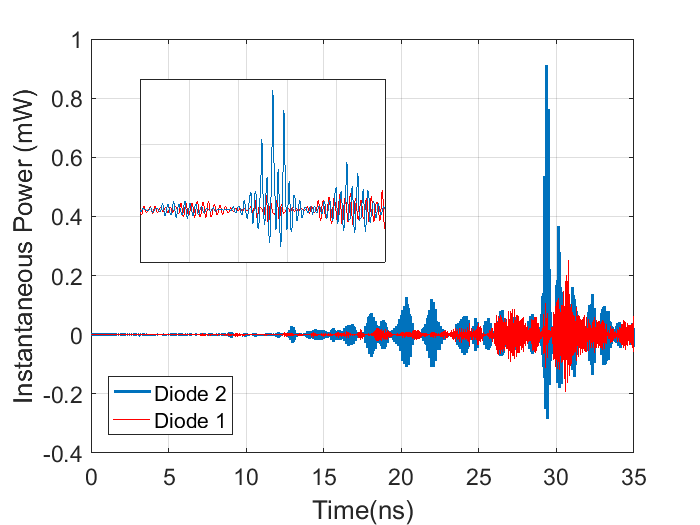
\includegraphics[width=\textwidth]{numerical/selective-recon-high}
\caption[Selective reconstruction on a $V_{k}^{high}$ diode]{Time-reversed reconstructions on the two diodes while targeting $V_{k}^{high}$. Sona amplitude modulation resulted in a clear contrast between the two signals.}
\label{fig:numerical-selective-recon-high}
\end{figure}

For this second scenario, with $V_k^{high} = 2.22V$, we once again used an amplitude $1.0 V$ pulse during the time-forward step so that we may compare the results from both scenarios equally. As shown in Figure~\ref{fig:numerical-selective-recon-high}, pulse amplitude of 1.0 has a maximum nonlinear response at $2.22V$. We chose this $V_k$ value as it gave the clearest reconstruction. Once again, we used pulse-inversion to extract the nonlinear sona. In general, this results in a larger magnitude reconstruction on $V_k^{high}$. This contrast between the $V_k^{low}$ and $V_k^{high}$ reconstructions was amplified by modulating the time-reversed sona amplitude, such that the reconstruction voltage seen at the target diode was barely larger than $V_k$ for $V_k^{high}$ and just barely smaller than $V_k$ for $V_k^{low}$. This resulted in selectively reconstructing on $V_k^{high}$ only during the time-reversed step with an aspect ratio of 3.61:1 for the $V_k^{high}$  diode relative to $V_k^{low}$, as shown in Figure~\ref{fig:numerical-selective-recon-high}.

\subsection{Discussion of Selective Nonlinear Time Reversal}

We have demonstrated a basic method for creating selective rectification using NLTR to target different nonlinear objects. This represents a stepping stone from the previously shown method of generalizing NLTR. By altering the input pulse amplitude, we were able to achieve the hypothesized nonlinear response suppression of specific nonlinear elements. This shows that the nonlinear reconstruction created on each nonlinear element is independent of one another and may be modified without impacting the other elements of the overall reconstructions. We have shown that this WPT technology would be capable of ubiquitous charging on any nonlinear device as well as selective targeting of specific devices. One may think of this as having an NLTR charger in one's home compared to having an NLTR in a business. In a domestic setting, there is very little need to restrict access to power. There are many outlets in one's home and there is no need to tell someone they are not permitted to use it. In a business however, a power outlet is not available to customers unless they pay for it. In this case, it is very useful to be able to selectively choose who may receive power. Although we have not shown a full-fledged system to do so, we have presented a foundational process that may be improved upon in order to create a successful NLTR-based WPT system.

\subsection{Simulation of Transmission Efficiency of NLTR Process}

We have so far shown that NLTR may be used in a WPT system to either power all nonlinear objects or selectively target the nonlinear objects within a relevant range. One significant question though that arises is to what efficiency are these objects powered. Surely a system that can only transfer 2\% of applied power will not be a successful WPT technology, as the consumer is paying for the luxury to not carry around a cable. If the user has to pay 50x more for the power they are very unlikely to use our system.
As previously discussed, energy losses are often difficult to calculate in real experiments due to wave reflection and other systematic sources of error. However, by simulating the NLTR process, we are able to observe approximate transfer efficiency. In CST, we are able to track input power and power loss via wave reflection, absorption in both lumped elements and environment materials, and radiation loss at other ports. One drawback to using the built-in CST power tracking is that everything is recorded in the frequency domain rather than time domain. For example, a typical power spectrum from a time-reversed step of a 2-diode NLTR simulation is shown in Figure~\ref{fig:numerical-power-spectrum}. As we are interested in overall power input compared to overall power output, we used this data along with Equation~\ref{eq:numerical-transfer-efficiency} to compute the efficiency of transfer in our simulations.

\begin{equation}
e = \frac{\sum_{i}P_{i(diode)}(f)}{\sum_{i}P_{i(input)}(f)} \cdot 100
\label{eq:numerical-transfer-efficiency}
\end{equation}

\begin{figure}[t]
\centering
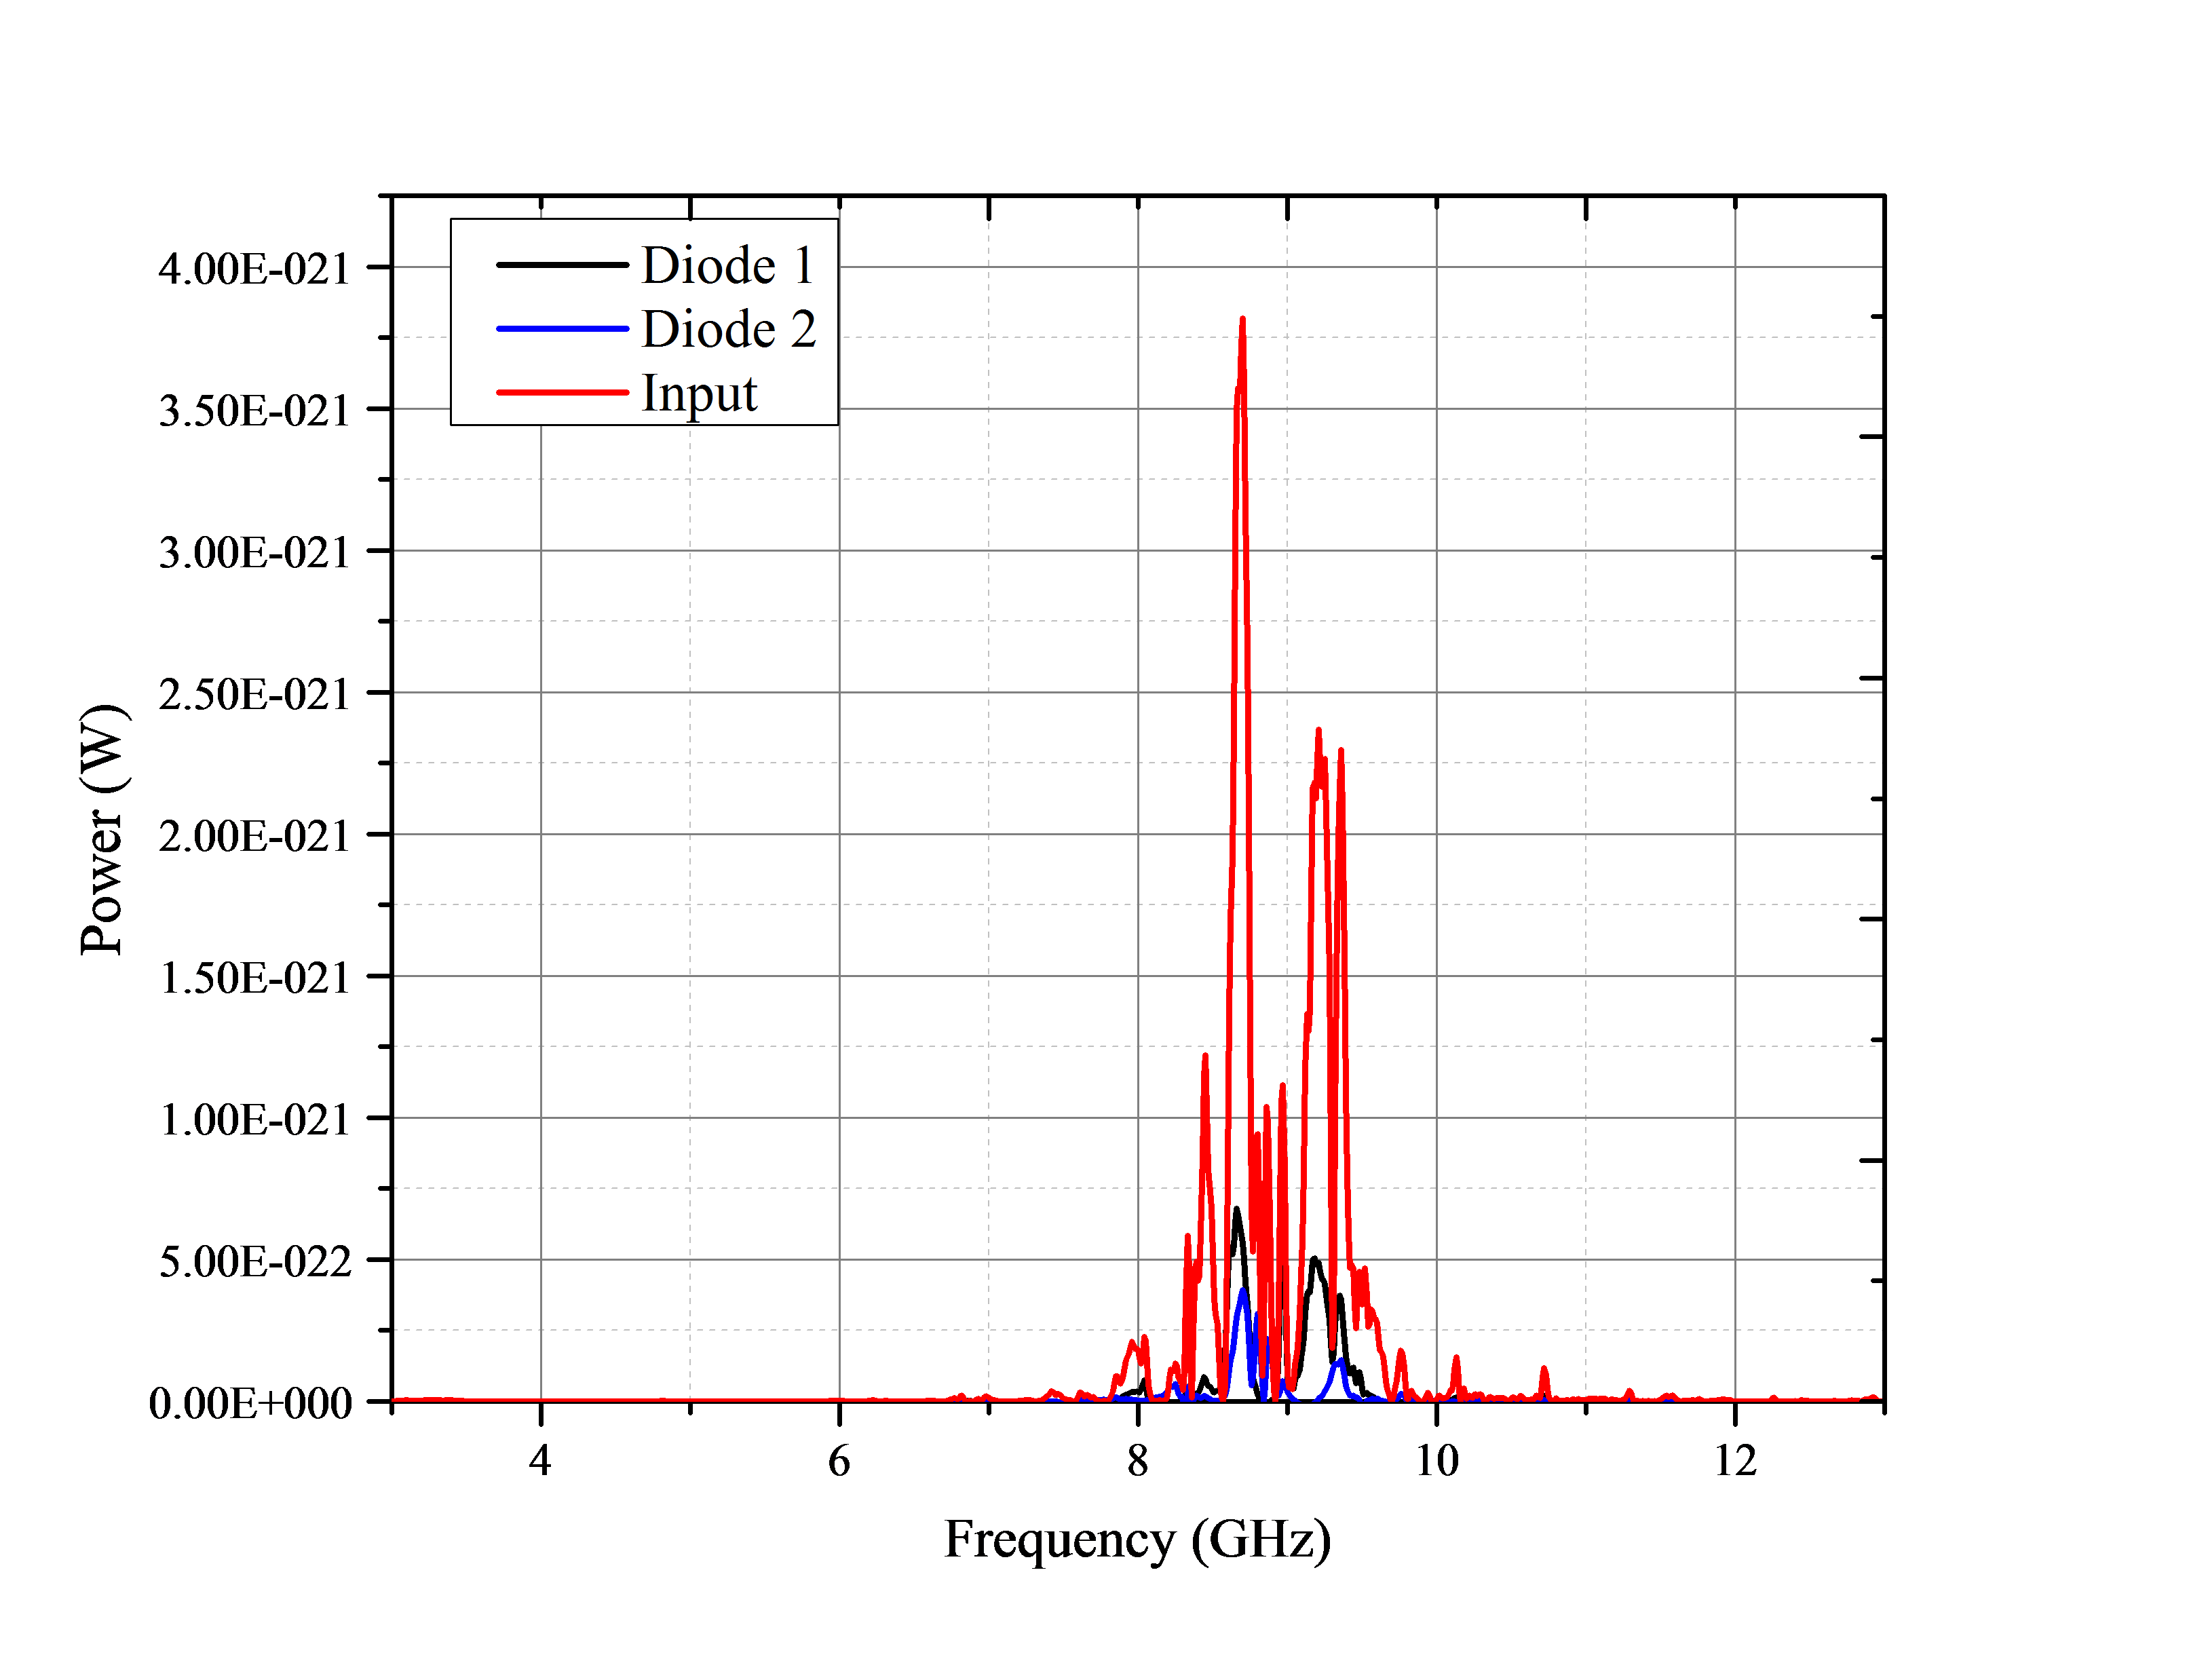
\includegraphics[width=\textwidth]{numerical/power-spectrum}
\caption[Transfer efficiency for a two-diode simultaneous reconstruction]{A typical power spectrum obtained in the time-reversed step (reconstruction). The power that enters the diodes only represents a portion of the overall power input in the simulation.}
\label{fig:numerical-power-spectrum}
\end{figure}

The above data was taken from a simulation in the Cut Box model for the previously discussed two-diode simultaneous reconstruction. For this simulation, we found that $18.6$\% and $7.3$\% of power were transferred from the nonlinear sona to diodes 1 and 2, respectively.  This provides a promising outlook.

Our next question was whether or not these transfer efficiencies were a function of distance between transmitter port, diode, and receiver port. We found that using similar diode positions as previously stated resulted in transmission values around the \numrange{7}{18}\% shown above. We decided to introduce a new model with a much larger length scale, called the Room Model shown in Figure~\ref{fig:numerical-room-model}.

\begin{figure}[t]
\centering
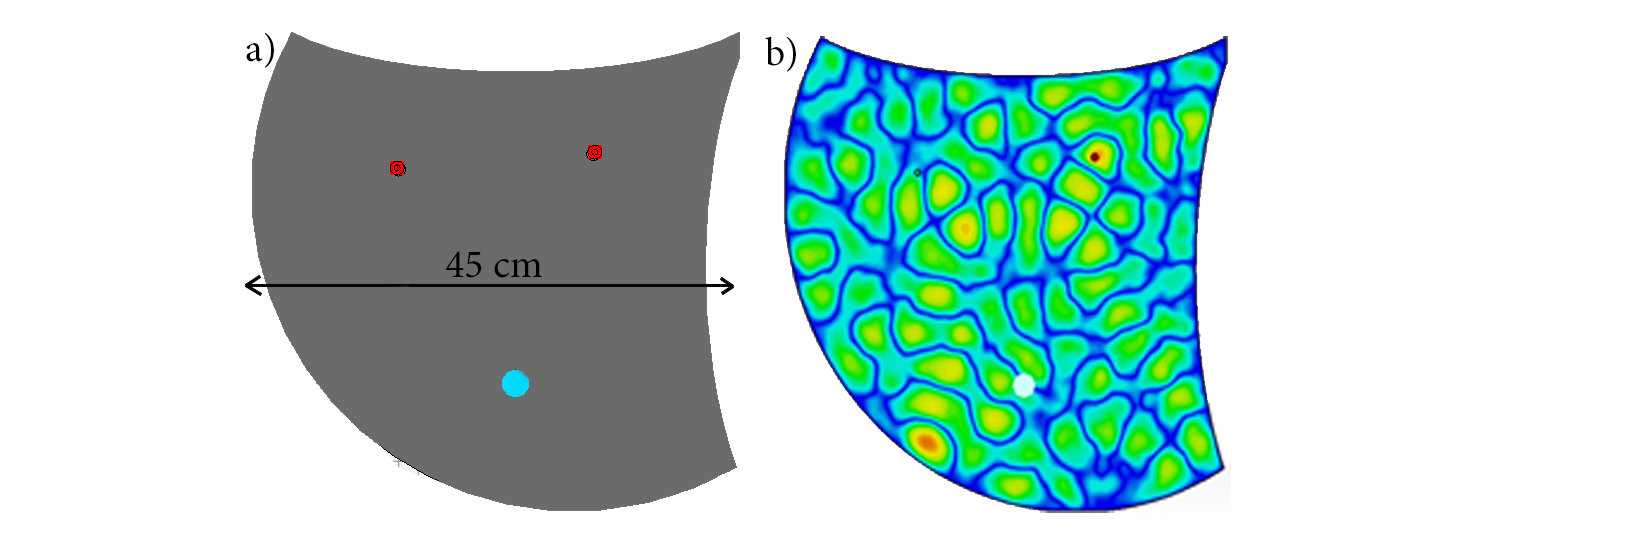
\includegraphics[width=0.85\textwidth]{numerical/room-model-a}
\caption[The Room Model]{(a) illustrates the geometry of the Room Model and (b)
shows the mode density of the space.}
\label{fig:numerical-room-model}
\end{figure}


We chose to use a 45cm x 45cm x 0.76 cm initial box to simulate a large geometry while still maintaining a quasi-2D cavity. The 45~cm length scale was used, as any larger simulation ran out of memory prior to completion.  Due to the length of simulation and decreased nonlinear signal strength, this model was unable to be used for further efficiency calculations. From Figure~\ref{fig:numerical-room-model}, the distances in the simulation are much larger than the Cut Box and may be used in the future to determine whether transmission efficiency of NLTR is dependent on distance between transmitter, nonlinear object, and receiver ports.

\section{Conclusion}
\label{sec:numerical-conclusion}

Using CST, we have successfully demonstrated our 3 goals: (1) simultaneous reconstructions on multiple nonlinear objects (2) selective reconstructions between multiple nonlinear objects and (3) calculation of a baseline transmission efficiency of NLTR. For simultaneous and selective targeting, we provide a basic framework to perform these processes using numerical simulations; however, these processes are still yet to be performed in real-world experimentation. We believe that this illustrates a foundational work for future experiments to demonstrate the feasibility of these features in a new WPT technology. Additional research must be done in order to characterize the ceiling on transmission efficiency if NLTR is to be applied to a future WPT technology.
